\documentclass[a4paper]{article}

\usepackage[utf8]{inputenc} %allows unicode (including russian) source file
\usepackage[russian]{babel} %docment in russian-style
\usepackage[utf8]{inputenc}
\usepackage[pdftex]{graphicx}


\begin{document}
    \begin{center}
        \begin{tabular}{|c|c|}
            \hline
            $ m $ & $ X_m, мм $ \\
            \hline
			-0.0999 & -4 \\
			-0.054 & -3 \\
			-0.0251 & -2 \\
			-0.0124 & -1 \\
			0.03 & 1 \\
			0.05 & 2 \\
			0.07 & 3 \\
			0.0914 & 42 \\
            \hline
        \end{tabular}
    \end{center}

    \begin{figure}[ht!]
    \centering
    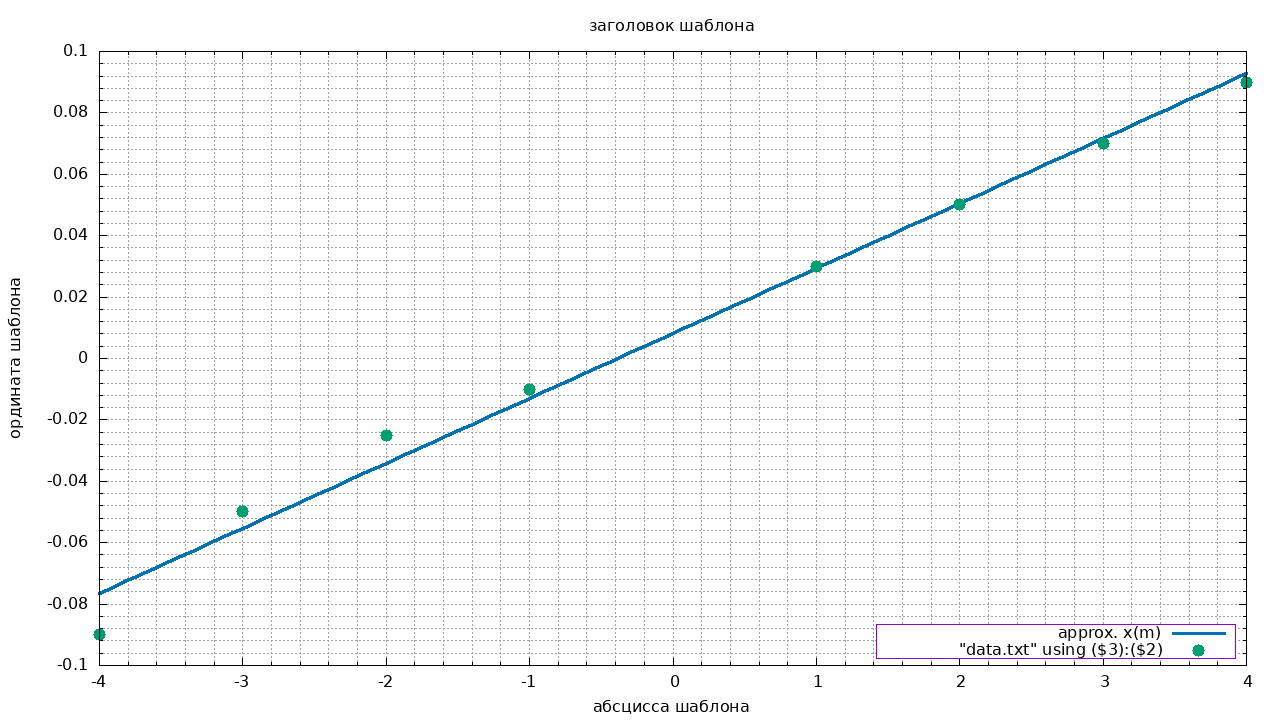
\includegraphics[width=100mm]{result.png}
    
    \caption{График зависимости смещения от числа m \label{overflow}}
    \end{figure}

\end{document}